\chapter{}
\section*{Из воспоминаний В.Б. Прейса}

Оказалось, что писать прозу мне значительно легче, чем воспоминания.

Во-первых, за много прошедших лет многое выветрилось из памяти и хронология событий сохранилась весьма примерно.

Во-вторых, поскольку дневников я никогда не вёл, то события в памяти восстанавливаются однобоко. Более хорошо вспоминаются взаимоотношения между мальчиками, а девочки остаются в стороне. Поэтому я стараюсь изложить то, что помню, но не исключаю возможных ошибок.

И, в-третьих, до какого времени нужно вспоминать? Мне кажется, что нужно закончить нашим окончанием школы, а всё остальное изложить в эпилоге. По моему мнению, каждый из нас должен написать свои воспоминания, а редактор или редколлегия должны это всё объединить, неважно если будут повторы, тогда может получиться цельная картина.

Итак, я начинаю вспоминать.

\indent

В Москве у Красных ворот, на пересечении Боярского переулка и Хоромного тупика, стоит шестиэтажный дом. Когда то он был серого цвета, а сейчас желтовато-лимонного. Этот дом был одним из первых кооперативных домов, построенных в Москве. В 1929 году он был заселен сотрудниками наркоматов иностранных дел и внешней торговли. В доме проживали ответственные сотрудники аппарата и несколько послов СССР в капстранах. Какое то время в нём жил Нарком иностранных дел М.М. Литвинов.

Дом был семиподьездный, в нём было 93 квартиры. Практически в каждой из них жили семьи с детьми, поэтому при доме функционировал детский сад. В Красном уголке иногда показывали кинофильмы, кроме того при нём работали кружки. Я помню два: автомодельный для старших ребят и драматический для младших.

Мне бы хотелось для полноты картины перечислить детей моего возраста, подростков и некоторых взрослых, которые мне запомнились.

В первом подъезде в квартире № 1 жила семья Яхниных с дочерью Лианой, очень серьёзной девочкой, моей ровесницей. В последствии она стала известным литературным переводчиком.

На втором этаже жили Варзары с сыном Севой и его младшей сестрой~-- Ксеной. Сева был отчаянный парень.
В последствии он воевал, был кавалером многих орденов и медалей, полковником артиллерии в отставке.

В пятой квартире жила семья Гриневских. Их старший сын Олег был нашим приятелем. В последствии он стал Чрезвычайным и полномочным послом, автором нескольких книг.

А в десятой квартире жили Бирюковы с рыженькой дочуркой Лилей и очень интересной мамой~-- Верой Исаевной. Уже будучи взрослым, я очень любил с ней беседовать. А с Лилей мы поддерживаем контакты и сейчас, хотя живем в разных городах США.

В 12 квартире жил Юра Богун. Он был несколько старше нас и был для нас большим авторитетом, он был наш главнокомандующий. Однажды он устроил манёвры. С криками Ура мы бежали на задний двор, а он со своего балкона сбросил на нас большую лампу от прожектора, которая разбилась с таким грохотом, что мы от страха разбежались. После этого его авторитет упал и мы, а вернее, он к нам, потеряли интерес.

На шестом этаже жила семья Меньшиковых. Дочка Таня и её брат Лева были несколько моложе меня. Не знаю почему, но мне доставляло удовольствие пугать их. Они начинали реветь и бежали домой, а вечером их мама Зинаида Борисовна звонила моим родителям и жаловалась на меня.

Во втором подъезде на первом этаже находился детский сад, который я посещал до поступления в школу.
Детский сад я помню весьма смутно. Единственно, что осталось в памяти, так это учительница немецкого азыка. Вернее даже не  она, а стишки, которые мы учили. Некоторые из них я помню и сейчас.

В квартире 23 жила Инна Веселовская, но она была старше нас, и  контактировать с ней мы уже начали после войны.

Двадцать четвертая квартира была многонаселенной. Как я слышал, в ней вначале жил доктор Петров. Когда его арестовали, оставалась жить его дочка. К ней подселился её дядя~-- Петров с женой и сыном Игорем, а потом в третью комнату этой квартиры вселился доктор Штернберг с сыном Шуриком. За достоверность изложенного я не очень ручаюсь, но и Игорь, и Шурик были нашими очень хорошими друзьями. В последствии Игорь стал инженером-электриком, кандидатом технических наук, а Шурик стал врачом-хирургом и женился на Лиле Бирюковой, что было дня меня неожиданностью. К сожалению, его уже с нами нет. Два годя назад он скончался к Америке.

В 26 квартире жила семья Плоткиных. По моему,  он был замначальнимка Правового отдела Наркомата иностранных дел и сгинул, как многие, в 38 году. У него остался сын Миша, но он был несколько моложе нас.

А в 28 квартире жила семья Андреевых, мать и взрослый сын. По-моему, в то довоенное время он уже преподавал в Вузе. К ним периодически приезжал её внук~-- Володя, который после войны долгое время жил у них. В последствии он стал Народным артистом, главным режиссером театра им. Ермоловой.

В третьем подьезде на третьем этаже жила семья Миниксов. Их было два брата, Марик, чуть моложе нас, и Аба, старший. Точного имени его я не знаю. Он погиб во время войны. А напротив жила семья Короткиных, их сын Жора тоже не вернулся с войны.

На третьем этаже в 36 квартире жили Дивильковские. Они приехали в наш дом наверное году в 3б, Их было два брата, Юра~-- старший и Сергей~-- наш ровесник.

Не знаю по какой причине, но до войны мы с ними не общались. Однако, в конце войны и все последующие годы 36 квартира, также как и Красный уголок, были нашим центром времяпрепровождения. Один Господь знает, каких усилий требовалось от Елены Васильевны~-- мамы Сергея, чтобы нас терпеть. В последующем Сергей Иванович Дивильковский работал на ответственных партийных и дипломатических должностях. Во время американо-вьетнамской войны был в Ханое. К сожалению, его старший брат во время войны погиб.

На четвертом этаже жил Миша Гюнтер. До войны мы с ним очень дружили, а потом наши пути как-то разошлись. Он примерно году в пятидесятом умер молодым.

На шестом этаже жили Лёнчнк Кузнецов и девочка Вайола Кофман, приехавшая в 35 году из Америки со своими родителями помогать строить социализм. Насколько я помню, девочка по-русски говорила лишь одно слово ~-- <<робяты>>. Потом она хорошо говорила по-русски, стала кандидатом наук. Сейчас она живет в Америке.

А Лёнчнк Кузнецов был основным моим <<противником>> во время игры в солдатики. В настоящее время Леон Дмитриевич работает в Москве. Он кандидат химических наук.

В четвертом подъезде на втором этаже жила Ирина Каменская~-- <<легендарная>> личность, но о ней несколько позже. Сейчас Ирина Ионовна живет в США. Насколько мне известно, написала комментарий к Библии и котируется в теологических кругах.

На третьем этаже в 47 квартире жили Кунины, приятели моего отца. У них было двое детей~-- Виктор и Ляля. Они были много старше меня.

Заметной личностью в этом подъезде был Штейн. Одно время он был послом в Италии, а позже~-- личным советником Молотова.

Напротив его квартиры жили Рабиновичи. Старший их сын Эмик был военным, а младший~-- Натик, хотя и был немногим старше нас, но с нами не общался. С ним я встретился в 1992 году в Израиле.

Интересным был пятый подъезд. На втором этаже жили Зивы. Их сын Миша подавал большие надежды в музыке. После ареста родителей, его не принимали в консерваторию; требовали, чтобы он отказался от родителей. Консерваторию он всё же окончил и стал довольно известным композитором. В 1980 г мне довелось с ним встретиться. Мы долго вспоминали дом и судьбы его жильцов.

Напротив квартиры Зивов жил Лоренц~-- посол СССР в Латвии. В 1937 г. он и его жена были арестованы и расстреляны. В их квартиру вселилась семья Иванцовых. Со старшим их сыном Сергеем я не дружил, а с младшим Игорем, любил играть. У него были очень красивые игрушки, по-моему, японские.

В квартире 59 жила семья Стомоняковых. Он был заместителем Наркома иностранных дел. Как я помню из разговора взрослых, когда его пришли арестовывать, он застрелился у себя в кабинете. Жену расстреляли позже.

На четвётом этаже жила семья Рубининых с двумя сыновьями, Павлом~-- старшим и Андреем чуть помоложе. Они появились а доме перед самой войной. Их отец был послом СССР в Бельгии. В 1950 г. его арестовали как еврейского националиста.

Напротив квартиры Рубининых была квартира Уманских. Они практически всё время жили в США, так как он был послом. У них была дочь Тита. Мы её знали, но видели редко. Где то в конце войны с ней случилась трагедия. Её застрелил сын Министра авиационной промышленности, чуть ли не на Красной площади.

Интересной была квартира 66. В ней вначале жил доктор Горелик. По рассказам, которые мне запомнились, он совершил гражданский подвиг. К нему на приём пришёл больной, у которого он заподозрил чуму. Горелик запер кабинет, вызвал спецмашину и она отвезла его и больного в инфекционную больницу, где они и скончались. Когда я уже был врачём, мне пришлось некоторое время работать с его братом С.Л. Гореликом, человеком с трудной судьбой.

После смерти Горелика в этой квартире поселился известный географ, писатель, путешественник~-- Лухманов.
С его внуком Димой до войны я дружил, а затем наши пути разошлись, и я встретился с ним уже будучи взрослым.

Напротив, в квартире 65, жила семья, которая туда вселилась после ареста прежних хозяев. Глава семьи был не то сотрудником НКВД, не то военным. У них был маленький ребенок. С ними же жила сестра жены молодая девушка по имени Маня. Видимо этот военный был очень ревнивый, а может быть был повод к тому, что он застрелил жену и себя. Маленького ребенка забрала бабушка, а Маня продолжала жить в квартире. Наш домуправ, Иван Максимович Калиш, который жил в первом подъезде в подвале, быстро сориентировался и поменялся с Маней. Дальнейшая её судьба была трудной, во время войны она стала доступной женщиной, а где-то к концу войны она поменялась с Медниковыми. Их сын Миша стел нашим близким товарищем. В последствии он защитил кандидатсскую диссертацию и стал инженером-атомщиком. Сейчас Михаил Исаакович Медников живет в Израиле.

В шестом подъезде в 71 квартире жили Первины. Во время войны их сын Илья попал в плен, бежал к партизанам, а потом был осужден на десять лет как изменник Родины.

Бывшая квартира Литвинова после его отъезда стала коммунальной и очень несчастливой. Сначала там жил некто Райвид. После его ареста в 37 году туда вселилась семья Досиков, а в 39 году арестовали и Досика. Кроме того, там жила семья Таракановых. С их дочкой Неллей мы дружили.

В квартире 78 до 37 года жили Мельниковы, а после их ареста туда въехала семья Пивень. Он был дипломатом и работал в Чехословакии. В 1939 году его тоже арестовали. У них в семье было две дочери~-- Алла и Мара. Алла была нашей подружкой, мы часто собирались у нее. В конфискованную комнату к ним вселили семью Горностаевых с двумя детьми. Старший Альберт стал нашим приятелем. К сожалению, Аллочка умерла из нашей компании первой, будучи самой младшей из нас.

В седьмом подъезде на втором этаже жили Линские. С их младшим сыном Славой до войны я дружил.

В 81 квартире жили Карские. Он был посол СССР в Эстонии. В 37 году его и жену расстелили. У них осталась одна дочь. А её дочь вышла замуж за Райского Юру, который жил этажом выше.

На третьем этаже жили Райские. У них был внук моложе нас. С его бабушкой после войны мы конфликтовали.

В 83 квартире жили Васильевы~-- тетя и дядя Шурика Штернберга. У них было двое сыновей. Старший Андрей и младший Костя. Шурик нас иногда приводил к ним и мы с удовольствием рассматривали электрическую железную дорогу.

В квартире 85 жили Рафаловские. Квартира была знаменита тем, что когда моя бабушка иногда приезжала к нам, она ходила к Рафаловским молиться. Кроме того, у них жила не то внучка, не то племянница Рита. Она была чуть старше меня, но мы с удовольствием играли друг с другом. А после войны она вдруг стала взрослой дамой и наши контакты прекратились.

В квартире 87 жил молодой военный с женой и трехлетней дочкой. Он был военным атташе, по моему, в Чехословакии. В одну из ночей 38 года их с женой арестовели, а маленькую девочку заперли одну в квартире. Наш дворник~-- Павел Сиротин, всегда бывший понятым при арестах, в эту ночь нашёл брата арестованного и тот забрал девочку к себе. О её дальнейшей судьбе мне ничего не известно.

На 5 этаже в 89 квартире жил бывший царский дипломат Соловьёв с супругой, по национальности немкой. Незадолго до начала войны Соловьёв умер, а в первые месяцы войны была интернирована его жена. Потом в эту квартиру вселили лётчика дальней бомбардировочной авиации. Когда он погиб, его вдова прописала у себя племянника. Я не знаю, что произошло в дальнейшем, но во время войны в квартиру въехала семья Ковалей. Он был начальником московского областного Управления уголовного розыска. У них было двое сыновей. Старший Борис и младший Юрий. С Борисом я учился в одном классе. Он всегда был душой общества и остается таким же по настоящее время. Закончив институт международных отношений, он не пошел по дипломатической линии, а стал учёным. Защитил докторскую диссертацию. Был директором НИИ международного рабочего движения. Сейчас Борис Иосифович Коваль~-- академик. Его младший брат Юра стал известным детским писателем. К великому сожалению, он рано умер. Где-то в конце войны они поменялись с Первиными и переехали в шестой подъезд.

А в 90 квартире жил я с родителями и старшей сестрой Розой. Поскольку она была много старше меня, то мне не возбранялось общаться и с ребятами её возраста, чем я и пользовался. Мое безоблачное детство закончилось в марте 1938 года, когда арестовали маму.

В 92 квартире жила семья Маковских. Они дружили с моим отцом. Сам Маковский был инженер, приехавший со своей женой Шарлоттой Августовной из Германин. Детей у них не было и они по доброму относились ко мне. Мне запомнился запах кофе и до блеска натертый пол. В 1933 или 36 году Маковского арестовали, но быстро освободили и у него, как говорили, была охранная грамота от самого Сталина. Но, несмотря на это, в 1938 году он был вновь арестован и сгинул в неизвестности. Жену же его, также как и Соловьеву, интернировали. Позже мы узнали, что её вывезли в Казахстан. 

Хочу рассказать одни эпизод, оставшийся у меня в памяти. Где-то около четырех часов утра 22 июня 41г. у нас раздался звонок в дверь. В то время этот звонок мог означать многое. Папа открыл дверь. На пороге стояла Шарлотта Августовна. Она отвела папу на кухню, что то ему сказала и ушла. Помню, что папа сказал ей, что этого не может быть. Когда мы его спросили, что случилось, он нам сказал, что Шарлотта слушала речь Гитлера, который сообщил о начале войны с СССР. Папа нас предупредил, чтобы мы никому не говорили об этом, а слушали радио, и днем мы услышали то, о чём говорила Шарлотта.

В 93 квартире жил Рональд Фишзон, он был отчаянным парнем. Году в 1940 он поступил в авиационную спецшколу, но во время войны воевал в пехоте. Был много раз ранен. Вернулся с большим числом наград. Кем он потом работал я не знаю, знаю лишь что под конец жизни он был директором турбазы на Памире.

В конце 1944 или в начале 1945 г. в 22 квартиру, в которой до 1941 г. жил Шейнинг (он был интернирован) вселилась семья Карпухиных. Мария Петровна~-- мама, прекрасная хлебосольная женщина, её сын Толя и дочь Зоя. Она была очень активной девочкой и быстро вошла в наш коллектив, также как и Лиля Бирюкова. В последствии она вышла замуж за нашего товарища~-- Володю Литвинова. Сейчас Зоя Фёдоровна Литвинова прабабушка и пытается воспитывать правнучку.

Ну вот я попытался вспомнить про наш дом и некоторых его жильцов, а теперь вспомним, что мы делали и чем занимались.

Безусловно, события, которые происходили в стране и в мире, мы без внимания оставить не могли. Мы были папанинцами, воевали с фашистами в Испании, летали с Чкаловым через Северный полюс, воевали на Хасане и протягивали руку братской дружбы жителям республик Прибалтики, Западной Украины, Белорусии и Молдавии.

В предвоенные годы мы, как правило, играли в войну. При станции метро <<Красные ворота>> был книжный магазин, в котором мы покупали книжки, имевшие прямое отношение к Красной Армии. Моей любимой книжкой был <<Устав вооружённых сил СССР>>. В 1936 году мне довелось быть с мамой на Первомайском параде на Красной площади. Всё, что я видел, произвело на меня огромное впечатление, особенно прохождение по площади с винтовками наперевес Пролетарской дивизии. Когда я рассказал ребятам об этом, мы пришли к мнению, что сильнее Пролетарской дивизии никого нет и она победит всех врагов. Тревожное положение, которое было в Мире, мы, естественно, не ощущали. Подошло время поступления в школу. Все мои сверстники поступили в школу в нашем районе, а меня записали мои родители в образцовую школу в другом районе, в котором работала моя мама. Мне приходилось туда ездить на трамвае, остановка которого была в конце скверика, где сейчас памятник Лермонтову. Я очень не любил туда ездить и всегда искал причину, чтобы прогулять.

А во дворе в подвалах почему-то начали строить бомбоубежища. Началась финская война. Она мне запомнилась двумя моментами. В моей образцовой школе развернули госпиталь, а нас перевели в далёкую школу да к тому же мы учились в третьей смене. Начинали в четыре и кончали в семь. Это было очень неприятно. Но второй момент был приятным. В том году была очень суровая зима и временами были сильные морозы. В такие дни школа была закрыта, а гулять во дворе нам никто не препятствовал, что мы с удовольствием и делали.

В мае 1941 года Слава Линский, Вайола Кофман, Лиана Яхнина и я закончили пять классов. Начался дачный сезон и многие дети разъехались. А мы в этом году дачу не снимали, так как болела моя тётя и ехать нам было не с кем.

Я прекрасно помню день начала войны. Это был солнечный воскресный день. По улицам, как всегда, ездили машины, трамваи, троллейбусы. Ходили люди. А в двенадцать часов по радио Молотов объявил, что началась война.

Во дворе дома стали собираться группами мужчины. Они были взволнованы, а мы думали, что они волнуются, ведь у нас есть Пролетарская дивизия, самая сильная в Мире.

На другой день наиболее старших из нас собрал домоуправ и повел всех на чердак. Наша задача заключалась в том, чтобы собрать весь хлам и отнести его к дверям. Взрослые забирали эти вещи и выносили их на улицу. Потом нам дали вёдра не то с известью, не то с мелом и кисти и велели красить деревянные балки. Мы всем этим были очень довольны. А домашние стали наклеивать на стекла крест-накрест бумажные ленты. Нам объяснили, что при взрыве бомбы это может сохранить стёкла.

Папа дома на стену повесил большую карту и чёрными и красными флажками отмечал ход боевых действий. Я удивлялся, Пролетарская дивизия отступала.

В один из дней поступило распоряжение сдать радио-приёмники и фотоаппараты, что мы и сделали.

Большую часть времени я проводил с ребятами на улице. Разнёсся слух, что около метро стоит Каганович. Мы побежали смотреть. Одет он был в форму железнодорожника и что-то говорил окружавшим его мужчинам, а затем с частью из них пошел в НКПС (Народный комиссариат путей сообщения), а мы сопровождали его. В последующие дни мы бегали на Чистые пруды. Часть деревьев там срубили, были вырыты окопы, в которых стояли зенитные пушки и пулемёты, а среди них ходили девушки в военной форме.

В городе была объявлена светомаскировка. Вечером не горели фонари, машины ездили с затемнёнными фарами, а в квартирах окна закрывались чем-либо черным.
По улицам ходили дежурные с противогазами на боку и очень следили за соблюдением светомаскировки. Но было лето, июнь, и на улице было светло.

Я уже не помню какое это было число, но был или глубокий вечер, или ночь, когда завыли сирены. Воздушная тревога. Папа оставался дома, а мы с сестрой пошли в метро, хотя в доме было два бомбоубежища. Очень неприятным был вой сирены, ещё и потому, что мы не знали настоящая это тревога или учебная. В метро почему-то нам пришлось спуститься на рельсы. Было очень грязно и душно. Плакали дети. Никто не знал, что делается наверху. Примерно через час был объявлен отбой и мы узнали, что тревога была учебной.

Мне лично очень досаждала школа, в которой я учился. Оттуда звонили нам домой, приходили и требовали, чтобы меня эвакуировали. Я отчаянно сопротивлялся и пока оставался дома.

Обстановка в городе становилась тревожной. Учреждения, которые располагались в нашем доме, эвакуировались. Сводки с фронтов были плохие. Учебные воздушные тревоги повторялись ещё несколько раз.

Но вот 22 июля, ровно через месяц после начала войны, ночью вновь завыли сирены. Мы подумали, что это опять учебная тревога. Но не успел ещё диктор закончить фразу: <<Граждане, воздушная тревога>> как послышались пулеметные выстрелы, а небо располосовали лучи прожекторов. Мы быстро побежали в бомбоубежище. После отбоя я со старшими ребятами пошел на Чистые пруды. Там девушки возились около пулеметов. На наши вопросы они не отвечали и велели идти домой. Кто-то сказал, что в районе вокзалов есть разрушения и взрослые ребята пошли туда, а я вернулся домой. Дома папа, он тоже был очень возбужден, рассказывал, что они действительно видели с крыши пламя в районе вокзалов, но наиболее сильные пожары были где-то в районе Серпуховки.

На следующую ночь или через ночь, я точно не помню, вновь была объявлена тревога. Я упросил папу, чтобы он взял меня на чердак. Там я встал под балкой у слухового окна. Стрельба и взрывы были довольно сильные. Было впечатление, что горит весь город. Взрослые говорили, что это горит лакокрасочный завод на Пресне. На крышу сыпалось большое количество осколков, некоторые из них пробивали железо и падали на чердак. Мужчины стояли под балками и прикрывали головы лопатами. Папа велел мне спуститься в убежище, вход в которое был около нашего подъезда. Я вышел во двор и перебежал в свой подъезд. Мне не хотелось спускаться в убежище и я остался стоять у дверей. Но в это время раздался такой силы взрыв, что мне показалось, будто дом подпрыгнул. Меня отбросило к одной стене, потом к другой и ... я не помню, как оказался в убежище. Меня спросили, что произошло снаружи и я ответил, что где-то близко от нас что-то взорвалось. После отбоя, дома папа сказал, что был очень сильный налёт, в городе много пожаров и где-то недалеко от нас взорвалась крупная бомба. Уже будучи юношей, из книги В. Лациса <<Буря>> я узнал, что по наводке немецкий лётчик сбросил бомбу большой мощности на здание Представительства Латвии, где в это время находилось всё Правительство республики. Это было на улице Чаплыгина, действительно довольно близко от нас.

Двор постепенно пустел, детей, практически, никого не осталось. И вот пятого августа бабушка, тетя, двоюродный брат и я отправились в эвакуацию. Уезжать мне не хотелось, но постоянные водушные тревоги и днём, и ночью, сделали своё дело.

Первый день нашего отъезда, а ехали мы в теплушках, ознаменовался неприятным эпизодом. К вечеру мы прибыли в Рязань. Наш эшелон остановился между воинским эшелоном, идущим на запад, и санитарным поездом, идущим на восток. Мы впервые увидели раненых. Вдруг раздался сигнал воздушной тревоги, а через некоторое время начали стрелять зенитки. Оба эшелона ушли по своим направлениям, а мы остались. У меня появилось такое чувство, что нас бросили. Через некоторое время всё закончилось и я успокоился. Последующий наш путь проходил без происшествий, если не считать, что я чуть не отстал от эшелона в Куйбышеве.

На пятые сутки мы прибыли на станцию Раевская Башкирской АССР. Эшелон разгрузили. Куда нас повезут дальше никто не знал. Кругом стояло много подвод. Нас посадили на одну из них и сказали, что мы едем в деревню Райны. Это недалеко~-- 60 км. Где-то ближе к вечеру нас и ещё четыре семьи привезли в эту деревню. Меня поразило, что крыши всех домов покрыты соломой, а не железом. К нашей подводе подошел мужчина и сказал чтобы мы ехали за ним. Вскоре мы подъехали к дому, из которого вышла молодая женщина и стала что-то говорить на непонятном языке. По её жестам мы поняли, что здесь мы будем жить. Дом был большой, но и семья у этой женщины была большая и конечно было тесно.

Через некоторое время мы с тётей нашли другой дом, где практически были одни. Его хозяйка, пожилая женщина Фатима-оби, жила на хуторе и приходила в дом редко. Единственная сложность для нас заключалась в том, что заготавливать дрова мы должны были сами. В отличие от других домов деревни, крыша у нашего дома была драночная, а не соломенная и, кроме того, он был огорожен деревянным забором, а не плетнём. Со стороны улицы у забора лежал большой камень, на котором мы любили сидеть. Хочу сделать небольшое отступление. В 1971 году, т.е. через тридцать лет после эвакуации, мне довелось посетить эту деревню. Деревня всегда была очень большой, а сейчас это стал просто агрогород. Большинство домов уже имело железные крыши, имелось электричество и радио, чего раньше не было. Единственно, что осталось неизменным, это непролазная грязь на улице. Так вот, я стал искать дом, в котором мы жили. Дома не было. Оказыватся он сгорел, но я узнал камень. Какой же он оказался маленький.

Единственным работником на первых порах был я. Это дало мне возможность научиться запрягать лошадь, косить траву, работать на сенокосилке, копать картофель, воровать на бахче арбузы, а на поле подсолнухи, но это было всё несколько позже.

В мои обязанности по дому входила доставка воды и я научился носить вёдра на коромысле, пилка и рубка дров, а также растапливание печи. Поначалу не всё получалось, но потом я освоился. Нам сказали, что Правление колхоза выдает эвакуированным муку. Нашей семье полагалось 20 килограмм, и за ней нужно было идти на другой конец деревни на склад. Сколько это 20 кг, ни мои родичи, ни тем более я, не представляли. Надо отметить, что я был довольно слабеньким, не высокого роста, мальчиком. Мне дома дали наволочку и я отправился за мукой. Я уже говорил выше, что грязь на улице была непролазной, и ходить по этой дороге было сложно даже без груза. На складе мне взвесили муку и помогли взвалить наволочку на плечи. Пошатываясь я вышел на улицу и через пару шагов мешок у меня свалился. Поднять его я не мог, а только переставлял шага на два. Я не знал, что мне делать, но ко мне подошла женщина и стала что-то говорить мне по татарски. Язык я, естественно, не знал, но понял, что она велит мне оставаться на месте и никуда не уходить. Она ушла и скоро вернулась с тележкой, помогла мне положить на неё наволочку с мукой и мы поехали. Через какое то время она показала мне дом. Я понял, что она здесь живет и сюда нужно вернуть тележку, что я и сделал. После этого я понял, что такое 20 кг. Я не буду описывать как мы жили в эвакуации~-- это тема отдельного повествования, скажу лишь одно, основной нашей пищей была картошка. Однажды с ребятами я охотился на голубей и нескольких принёс домой. В этот день мы ели голубиный суп.

В конце октября 1941 г. к нам приехали из Москвы папа, сестра и папин брат. Мужчины пошли работать и жить нам стало полегче.

В начале 1942 г. к нам из госпиталя приехал папин младший брат. У него была тяжелейшая контузия и он долго лежал в Свердловске в госпитале. В конечном счёте он был признан негодным к службе в армии. По состоянию здоровья в колхозе он тоже работать не мог. Через некоторое время они с папой решили вернуться в Москву, но папу не пропустили и он возвратился к нам. Где-то в апреле 1943 г. Папа съездил в Уфу и ему удалось устроиться там на работу. Он вернулся за мной и пятого мая, эту дату я очень хорошо запомнил, мы приехали в Уфу. У папы уже были продовольственные карточки и около вокзала мы их <<отоварили>> как тогда говорили, купив пять килограмм хлеба. Пока мы дошли от вокзала до дома, где нам предстояло жить, хлеба у нас уже не было.

Я уже упоминал, что перед войной я закончил пять классов. В деревне я не учился, так как там была только четырехлетка, да и та на татарском языке, поэтому я пропустил два года. В Уфе я пошел учиться в шестой класс. От школы я отвык и мне было несколько трудновато, однако учился я неплохо.

В январе мы получили пропуск и вернулись в Москву. Мы приехали как раз в период школьных каникул, меня записали в 310 школу и десятого января я пошёл учиться. Школа была только для мальчиков, сколько нас было в классе я не помню. Первый день ознаменовался для меня двумя событиями. Мы писали диктант и к моему удивлению и ужасу я сделал тринадцать ошибок, причём одна была нелепее другой. Из всех ребят в классе мне запомнился один. Он был очень активный, гонялся за кем-то по классу и в конце концов с учительского стола сбросил чернильницу на пол, которая, естественно, разбилась. Пришла учительница, вызвала директора по кличке <<Бегемот>> (он был очень толстый). Естественно первым вопросом был : <<кто это сделал?>> Ответа не последовало. Тогда директор сказал: <<Будете сидеть до тех пор, пока не сознаетесь. Принесите им ведро,~-- сказал он нянечке,~-- и заприте дверь класса>>. Всё было выполнено. Сознаваться никто не собирался и все были рады, что занятий не будет. А с мальчиком, который разбил чернильницу, я подружился, его звали Володя Литвинов.

Стало темнеть, мы зажгли свет в классе и потянулись к ведру. Стали появляться родители. Наконец пришли и за мной, а за Володей никто не приходил. Позже я узнал, что через некоторое время всех оставшихся директор отпустил.

А во дворе было уже много ребят и мы практически все учились в одной школе. И девочки тоже учились все вместе. Среди мальчиков появился новенький~-- Боря Коваль и присоединился Серёжа Дивильковскмй.

Мне запомнился один эпизод, относящийся к этому времени. В начале июня 1944 г. по Москве должны были провести пленных немцев. Как назло, в этот день утром у нас был экзамен по алгебре. Но мне было не до алгебры, мне очень хотелось посмотреть на немцев. Экзамен был устным и что я там наболтал, не помню. Но получив оценку, тут же побежал на Садовое кольцо. Немцев я не пропустил.

Нашим ребячьим увлечением в это время был футбол. Рядом с нашим домом находилась довольно приличная площадка, которую по чьей-то хорошей идее назвали Папанин-бридж. Причин для названия было две. Говорили, что в доме, где была эта площадка, жил Папанин, а слово бридж было присвоено потому, что команда московского <<Динамо>> совершила триумфальное турне по Англии. Так вот этот Папанин-бридж на многие годы стал для нас центром притяжения. Кроме того, мы выезжали играть в футбол и за город. Чаще всего в Болшево. Противниками нашими были ребята из соседнего дома, У них было два очень сильных игрока~-- Володя Епишин и Коля Фролов. Кто был ещё в их команде я не помню, но честно признаюсь~-- они играли лучше нас. И мне как вратарю это было особенно известно.

С девочками у нас в это время особых контактов не было.

Я уже упоминал, что в доме был Красный уголок. Практически каждый вечер мы там собирались, играли в биллиард или просто дурачились. Но мы становились старше. Появился патефон, стали приходить девочки. Я притащил из дома флирт и началась переписка. Почему-то на память приходит такая сентенция:

<<Лютик: Маргаритка, вы мне нравитесь! И следует ответ: Все мужчины крокодилы!>> А чуть позже мы уже стали собираться у Аллочки Пивень или у Люции Фроловой дома. Традиционной едой был винегрет. Не обходилось и без выпивки. Любимое вино~-- три семерки.

Следует отметить, что мы жили достаточно вольной жизнью. Родителям было как то не до нас. Но мне хотелось бы подчеркнуть, что ничего предосудительного мы
себе не позволяли.

Кому первому в голову пришла мысль об объединении всех нас, проживающих в разных домах в <<Союз>>, я не помню. Мне кажется, что Игорю Петрову, но как бы то ни было, в 1947 году был создан Союз Соединенных Домов~-- ССД. Тайным голосованием (по моему голосовали одни мальчики) был избран Президент~-- Сергей Иванович Дивильковский, Председатель Совета Министров, он же Министр финансов~-- Олег Алексеевич Гриневский и Министры: Министр Вооружённых сил~-- Борис Иосифович Коваль, Министр внутренних дел~-- Александр Александрович Штернберг, Прокурор~-- Владимир Матвеевич Литвинов, Министр Кинематографии, он же редактор журнала <<Вундеркинд>>~-- Виктор Борисович Прейс. Кроме того, у нас был свой собственный Патриарх и по совместительству Муллейшнй, Буддейший и Раввинейший~-- Игорь Михайлович Петров. Все остальные были граждане ССД, только лишь Зоя Фёдоровна Карпухина присвоила себе звание женделегатки от второго подъезда.

Одновременно с образованием ССД стал выходить журнал <<Вундеркинд>>. Когда я сейчас просматриваю его меня поражают две вещи. Во-первых, жуткое количество грамматических ошибок (а ведь я был его редактором под фамилией Кебзак), и, во-вторых, то, что мы там писали, по тем временам тянуло на 58 статью УПК. И хотя прямой антисоветчины не было, но многие вещи преподносились как пародия, как насмешка над действительностью. Однако мы, в силу своей дурости, над этим не задумывались.

Итак, в 1947 году было создано Государство, объединившее значительное число мальчиков и девочек со всей округи. Например, Томочка Зайцева жила на Чистых Прудах, а Миша Стояновский на Сретенке.

Как и положено Государству, мы имели свой Гимн. Автором его был Игорь Петров, а музыка была взята из модного тогда кинофильма <<Девушка моей мечты>>. Ниже я привожу слова Гимна:

\indent

{\itshape

Славься, славься государство наше.

Самая прекрасная Страна,

Ты всех стран сильней, могуче, краше.

Круглый год в тебе стоит весна.

\indent

Славься, славься ССД вовеки.

Демократия в тебе сильна! 

Здесь живут свободно человеки! 

Круглый год в тебе стоит весна.

\indent

В ССД вся власть в руках народа.

Много в нём закусок н вина.

В ССД господствует свобода!

В ССД всегда стоит весна!
}

\indent

Конечно, то, что писалось в журнале, было очень наивным. Но журнал ждали и читали с удовольствием. С моей точки зрения, были и хорошие стихи и рассказы. Одним из таких стихотворений было стихотворение, написанное Сергеем Дивильковским под псевдонимом С. Тютюн-Брджиевскнй. Я привожу его с некоторым сокращением. Называлось оно <<Московские рынки>>.

\indent

{\itshape

Трубная площадь. Центральный базар,

Скверик, трамваи, милиция.

Шум деловой. Цветной бульвар.

Вопли обманутых. Жизнь многолицая.



Был я в Берлине, гулял по аллее 

Unter den Linden~-- красиво! Картинка!

Но об одном я серьезно жалею.

Нету в Берлине хорошего рынка.



Наш бы московский немецкий рынок 

Взять бы, да к немцам в логово.

Да, а то что это? Как ботинок 

Для человека безногого.




Эх, вот Москва! Исторический запах. 

Преображенка. Дух истории.

Будто в Петровых огромных лапах 

Две столицы из-за рынка спорили.

Стой и любуйся! Год ли, час ли,

Минуту стой или две.

Как вы, не знаю, а я лично счастлив,

Что проживаю в Москве!
}

\indent

Журнал мы издавали ровно год, а потом вынуждены были прекратить. Причина тому была следующая. Двенадцатый номер журнала мы принесли в школу на вечер и там его либо потеряли, либо его кто-то специально передал директору. В разгар вечера меня вызвали к нему в кабинет. Там сидело довольно много учителей. Меня спросили, наш ли это журнал. Я ответил утвердительно, поскольку там были наши имена и фамилии. Должен сделать небольшое отступление. Учился я слабо, моими основными оценками были тройки. Директор мне сказал:

Виктор! Лучше потрать твои мысли и фантазию на учебу, а не на журнал.

Конечно этот разговор был мне неприятен, тем более, что моя биография была подмоченной. После этого выпуск журнала прекратился.

Однако у Олега Гриневского есть другая версия, будто пионервожатая из школы Аня Кулагина вызвала его и сказала, что надо кончать это дело, иначе могут быть большие неприятности. Он нам сказал об этом и мы перестали выпускать журнал. Я лично такого факта не помню.

Пережили мы и ещё один неприятный момент. Но Все по порядку. Наш очередной домоуправ~-- Александра Никитична со своей дочкой жила в Красном уголке. Она не очень препятствовала нам, когда мы там находились. В томже Красном уголке на тумбе стоял бюст Сталина. В один из вечеров мы уж очень расшумелись и разбегались и кто-то зацепил эту тумбу, она закачалась. Мы остолбенели. Вдруг бюст вождя, а он был гипсовый и покрашен под бронзу, упал на пол и с жутким грохотом разбился. Из своей комнаты выскочила Александра Никитична, увидела это дело и полушёпотом нам сказала:

\textit{Всё на задний двор и в пыль.}

Мы выполнили её распоряжение и всё, что было ранее Вождём, превратили в пыль.

Но не всегда наши отношения с Александрой Никитичной были ровными. Иногда мы ей надоедали и она выгоняла нас, запирая изнутри дверь. В один из таких эпизодов, она нас всех выгнала, но Камека (Ира Каменская) спряталась, через некоторое время открыла нам дверь и мы снова захватили Красный уголок. По этому поводу Сергей написал балладу: <<О взятии Красного уголка>>. Кроме всего, там были такие слова:

\indent

{\itshape
А главная осады героиня, храбрее не сыскать нам человека, зволась она де Лякруа ~-- графиня, а попросту, по нашему, Камека!
}

\indent

Так вот о Камеке. Настало такое время, когда мы стали обращать внимание на девочек, а они на нас. Меня любила Люция, Шурик любил Ксену, а Боря Таню Меньшикову. Но наши отношения были очень чистыми. А Камека страстно любила Володю Литвинова. Но это не мешало ей утверждать, что она никогда не поцелуется с мальчиком. Но к нашему изумлению (девочкам наверное это было известно) первая вышла замуж. Но самое примечательное в другом. На утро после первой брачной ночи, она в красивом, по моему в голубоватом, платье, выбежала во двор, стала бегать и кричать <<Я женщина, я женщина !>> Это было очень забавно.

Уже здесь, в Америке, я связался с ней и предложил тоже написать свои воспоминания, но она отказалась, ссылаясь на занятость. Но в то же время рассказала мне, что когда она вышла замуж и в дневное время занималась с Сеней любовью, со двора неслись крики: <<Зоя - штандер, Игорь - штандер>>, но это их не отвлекало.

А потом мы закончили школу, практически все поступили в институты и на этом наше отрочество закончилось.
Какое то время ССД существовал лишь номинально. Иногда небольшими группами мы собирались, но массовых сборов не было.

А через 40 лет мы собрали весь ССД. В гостинице <<Интурист>> был устроен банкет и выпущен юбилейный номер Вундеркинда. После этого вечера периодически мы стали собираться, чаще всего у Люции. Это были приятные вечера.

А жизнь шла своим чередом. Уехали в Америку Камека, Лиля с Шуриком и я с Галей. Миша Медников уехал в Израиль

К сожалению, появились у нас и потери. Первой ушла от нас самая молодая~-- Аллочка Пивень, потом Воля Голубев и Миша Стояновский, а недавно и Шурик Штернберг~-- светлая им всем память.


\begin{figure}[h!]
    \thisfloatsetup{capbesideposition=left}
    \fcapside[\FBwidth]{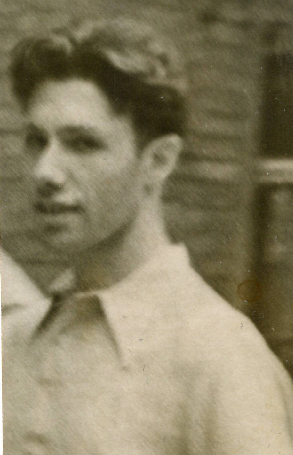
\includegraphics[height=70mm]{inc/preis}}{    \caption{Витя Прейс во дворе нашего дома. Начало пятидесятых.}}
    

\end{figure}